\chapter{Simulation studies for proton computed tomogrophy}



\section{The simulation software Allpix$^2$}
Allpix$^2$ is a generic simulation framework developed at CERN to simulate the performance of silicon detectors and was released in 2017. It builds upon the
Geant4 \cite{geant4} package to perform tasks in the simulation chain. The main tasks of Allpix$^2$ is the simulation of energy depostions of particles
in the sensors, the propagation of charge carriers in the sensor material and the digitization of the signal. It has a modular
structure to ensure an easy handling, while still allowing for complex detector simulations. Instantiation and processing of the modules is done by the core of the framework,
which contains five subsystems. This includes the configuration containing the configuration manager, which grants access to the configuration file, the
module subsystem, which loads and executes the modules and the geometry subsystem, which provides the information of the telescope setup. Objects are transferred
from one module to another with the messenger subsystem.
Figure \ref{fig:allpix} depicts the overall structure of Allpix$^2$.

\begin{figure}
  \centering
  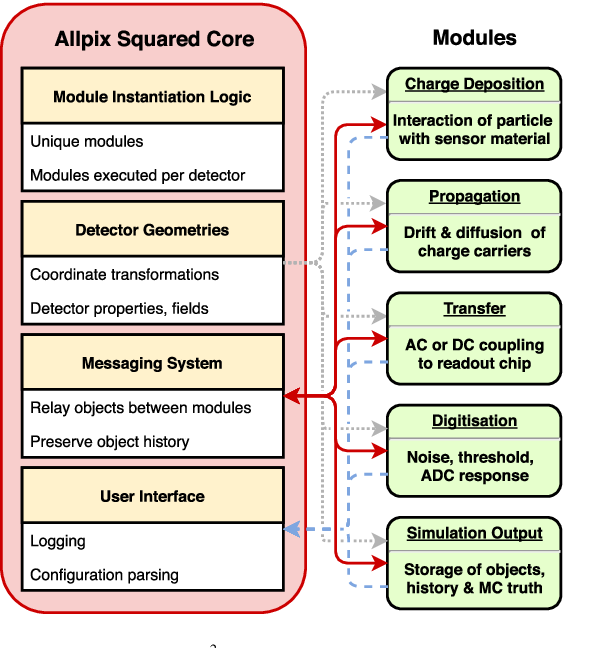
\includegraphics[height=0.5\textwidth]{images/allpix.png}
  \caption{Schematic representation of the overall Allpix$^2$ structure. \cite{fig_allpix}.}
  \label{fig:allpix}
\end{figure}

The telescope geometry has to be specified in a geometry file, which includes all sensors and their pixel matrix as well as their spatial and time resolution. Additionally,
the position and orientation have to be stated. Optionally, uncertainties on the position and orientation can be set to account for misalignment in real telescope setups.
In the configuration file, the geometry is imported as well as the modules for the simulation in order of execution, which
will be explained in the following.

The world frame of the simulation is created with the GeometryBuilderGeant4 module. The world material can be either air or vacuum with a configurable world margin percentage.
Afterwards all detectors from the internal detector models and passive material models are created according to the specifications in the geometry file.

Charge carriers are deposited in the active volume with the DepositionGeant4 module, which initializes the simulation of particles. The shape of the source beam, as well
as the type of particle and its energy can be specified. Further parameters are the width of the beam, its angular distribution based on a gaussian distribution and the energy
uncertainty of the simulated particles. All particles created at the same time define an event. The number of generated electron hole pairs is calculated with the
mean pair creation energy and is subject to fluctuations, which are defined by the fano factor.

An electric field is added to the sensors with the ElectricFieldReader module. By default all sensors are targeted by the module, though specific sensors can be stated.
There are three types of electric field models available, constant electric fields, linear electric fields and external simulated electric fields, with only
linear electric fiels being used in the scope of this thesis. The constant slope of linear electirc fields are defined by the bias voltage and the
depletion voltage of the sensor. Optionally, the depletion depth instead of the depletion voltage can be specified.

Either with the ProjectionPropagation or the GenericPropagation module the transport of charge carriers through the sensitive material are simulated.
The first module projects electrons or hole onto the surface and performs a randomized diffusion based on a two dimensional gaussian distribution around
the projection. Using an approximation of the drift time makes it possible to determine the diffusion width under the assumption of a linear electric field. This
module save computing time at the cost of accuracy. \\
The GenericPropagation module consists of a combined simulation of diffusion and drift calculated with a Runge-Kutter-Fehlberg method.
It is compatible with any electric field model and can simulate both electrons and holes
at the same time making the module
more accurate at the cost of computing time. The integration time can be specified by the user to determine the time of the propagation process. \\
In both modules, charge carriers are combined to sets and propagated together with no interaction between them. The set size of charge carriers can be specified by the user,
making it possible to control the accuracy and computing time of the simulation. For diffusion simulations it is necessary to specifiy the temperature of the sensor material
to calculate the diffusion constant.

Sets of charges are combined on the sensor pixels with the SimpleTransfer module and are prepared  to be processed by the front-end chips. The
propagated charges are mapped directly to the nearest pixel, while charge carriers that are outside the pixel grid or too far away from the implants are ignored.

Collected charges are then translated into digitised signals proportional to the input charge by the DefaultDigitizer module. Additionally, gaussian noise constributions
from the readout electronics can be simulated and a signal threshold can be defined. The output signal is given in units of the electron charge per default, but
can also be given in bits by simulating a QDC converter. Optionally, a gain factor and gain smearing can be set.

Simulated events and the produced plots of the different modules are stored in a root file. With the ROOTObjectWriter module further information like propagated charge,
deposited charge, Monte Carlo (MC) particle information and pixel hit information are stored in an additional ROOT file. Allpix$^2$ also enables the storing of
data in formats compatible with the EUTelescope and Corryvreckan software with the LCIOWriter module and the CorryvreckanWriter module respectively. Both modules possess parameters, which
determine what information of the Allpix$^2$ simulation is written into the ROOT files.
